\documentclass[bare_jrnl_transmag]{subfiles}
\begin{document}

\subsection{Kalman Filter Performance}
The performance of the Kalman Filter was validated by plotting the output of the filter against the ground truth position of the drone in the world frame. The ground truth position was parsed from the dataset, and the Kalman Filter was run on the raw sensor data, also parsed from the dataset. Using Matplotlib, both of these results were plotted on a 3D graph, with the x, y and z axes representing the world frame. The Kalman Filter output was plotted in orange, while the ground truth was plotted in blue. 

\begin{figure}[H]
    \centering
    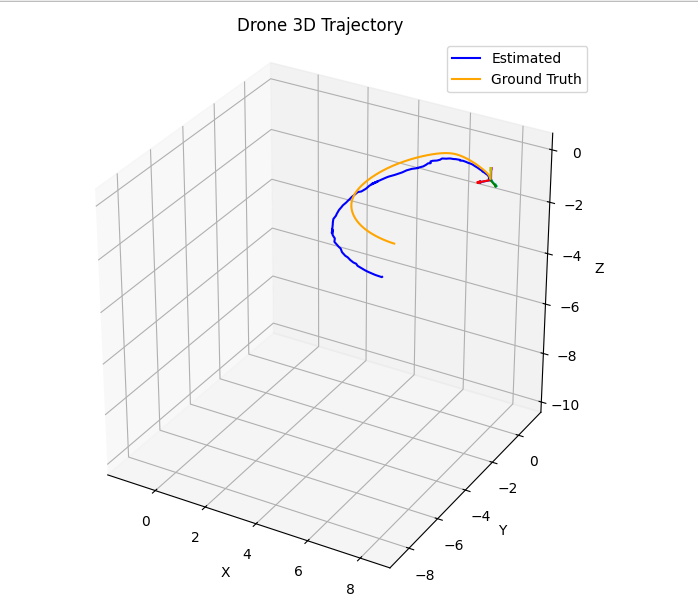
\includegraphics[width=0.8\linewidth]{figures/ekf_results.png}
    \caption{Kalman Filter results. The blue line is the ground-truth pose of the drone, while the orange line is the pose angle estimated by the Kalman filter.}
    \label{fig:kalman_results}
\end{figure}

It is observed that although the ground truth is tracked very well by the filter, there is observed drift, particularly on the z-axis. The Kalman Filter was tuned using the process and measurement noise matrices, which were iterated upon with different values to find the best fit. Ultimately, the filter was tuned to get an RMSE of [6.67, 5.41, 1.06] for the x, y and z axes respectively.

\end{document}